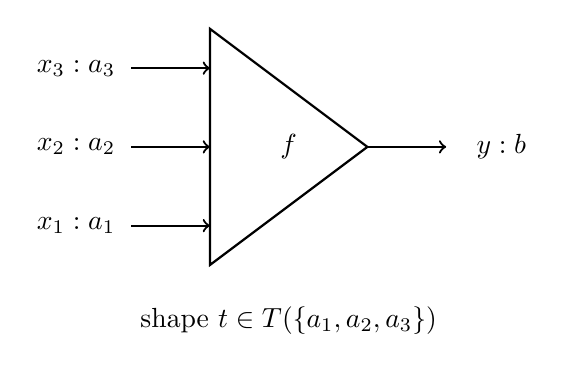
\begin{tikzpicture}
    % Draw the triangle with vertical left edge
    \draw[thick, fill=white] (0,0) -- (0,3) -- (2,1.5) -- cycle;

    % Draw input arrows
    \draw[->, thick] (-1,0.5) -- (0,0.5);
    \draw[->, thick] (-1,1.5) -- (0,1.5);
    \draw[->, thick] (-1,2.5) -- (0,2.5);

    % Draw output arrow
    \draw[->, thick] (2,1.5) -- (3,1.5);

    % Add labels
    \node at (1,1.5) {$f$};
    \node at (-1.7,0.5) {$x_1: a_1$};
    \node at (-1.7,1.5) {$x_2: a_2$};
    \node at (-1.7,2.5) {$x_3: a_3$};
    \node at (3.7,1.5) {$y: b$};
    \node at (1,-0.7) {shape $t \in T(\{a_1, a_2, a_3\})$};
\end{tikzpicture}